\documentclass[tikz,border=8pt]{standalone}
\usepackage{amsmath}
\usetikzlibrary{arrows.meta,decorations.pathmorphing}
\definecolor{ink}{HTML}{21352F}
\definecolor{teal}{HTML}{087F7B}
\definecolor{blue}{HTML}{4B77A8}
\definecolor{gold}{HTML}{C58B2A}
\definecolor{rose}{HTML}{B65A62}
\begin{document}
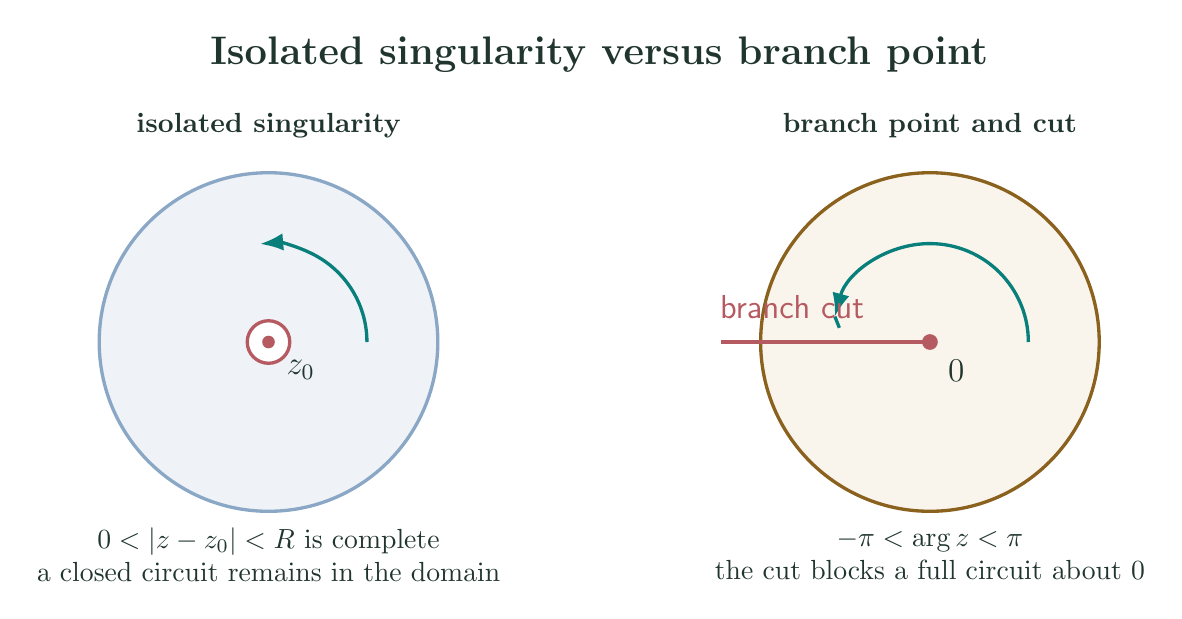
\begin{tikzpicture}[font=\large\sffamily,text=ink,>=Latex]
  \node[font=\bfseries\Large] at (0,3.65)
    {Isolated singularity versus branch point};

  \begin{scope}[xshift=-4.2cm]
    \node[font=\bfseries] at (0,2.75) {isolated singularity};
    \fill[blue!9] (0,0) circle (2.15);
    \draw[blue!65,very thick] (0,0) circle (2.15);
    \fill[white] (0,0) circle (.27);
    \draw[rose,very thick] (0,0) circle (.27);
    \fill[rose] (0,0) circle (.08);
    \node[below right=3pt] at (0,0) {$z_0$};
    \draw[teal,very thick,->] (1.25,0)
      arc[start angle=0,end angle=95,radius=1.25];
    \node[align=center,font=\normalsize] at (0,-2.7)
      {$0<|z-z_0|<R$ is complete\\
       a closed circuit remains in the domain};
  \end{scope}

  \begin{scope}[xshift=4.2cm]
    \node[font=\bfseries] at (0,2.75) {branch point and cut};
    \fill[gold!9] (0,0) circle (2.15);
    \draw[gold!70!black,very thick] (0,0) circle (2.15);
    \draw[rose,very thick] (-2.65,0)--(0,0);
    \fill[rose] (0,0) circle (.1);
    \node[below right=3pt] at (0,0) {$0$};
    \draw[teal,very thick,->] (1.25,0)
      arc[start angle=0,end angle=165,radius=1.25];
    \draw[teal,very thick] ({1.25*cos(165)},{1.25*sin(165)})
      --(-1.15,.18);
    \node[rose,above=5pt] at (-1.75,0) {branch cut};
    \node[align=center,font=\normalsize] at (0,-2.7)
      {$-\pi<\arg z<\pi$\\
       the cut blocks a full circuit about $0$};
  \end{scope}
\end{tikzpicture}
\end{document}
